\documentclass[11pt,a4paper]{report}
\usepackage[utf8]{inputenc}
\usepackage[russian]{babel}
\usepackage[OT1]{fontenc}
\usepackage{amsmath}
\usepackage{amsfonts}
\usepackage{amssymb}
\usepackage{graphicx}
\author{Григорий Субботин, Кирилл Муратов, Света Горбунова}
\title{Документация по проекту easySpace}
\begin{document}

\begin{titlepage}
 \begin{center}
    \large
    МИНИСТЕРСТВО ОБРАЗОВАНИЯ И НАУКИ\\ РОССИЙСКОЙ ФЕДЕРАЦИИ
     
    \textit{ФГБОУ ВО Российской Федерации}
    \vspace{0.5cm}
 
    АЛТАЙСКИЙ ГОСУДАРСТВЕННЫЙ УНИВЕРСИТЕТ
    
    \vspace{0.25cm}
     
    \textit{Институт цифровых технологий, электроники и физики}
    
    \vfill 
    Информатика и вычислительная техника
    \vfill
    \textsc{Групповая работа}\\[5mm]
     
    {\LARGE «Разработка графической программы с использованием библиотеки Tkinter, моделирующую солнечную систему»}
  \bigskip
     
     2 курс, группа 595
\end{center}
\vfill
 
\newlength{\ML}
\settowidth{\ML}{«\underline{\hspace{0.6cm}}» \underline{\hspace{1cm}}}
\hfill\begin{minipage}{0.5\textwidth}
  Руководитель курса\\
  \underline{\hspace{\ML}} И.\,А.~Шмаков\\
  «\underline{\hspace{0.5cm}}» \underline{\hspace{1cm}} 2020 г.
\end{minipage}%
\bigskip
 
\hfill\begin{minipage}{0.5\textwidth}
  Студенческая группа:\\
  \underline{\hspace{\ML}} Г.\,М.~Субботин  \\- менеджер проекта\\
  \underline{\hspace{\ML}} К.\,М.~Муратов \\- кодер\\
  \underline{\hspace{\ML}} С.\,М.~Горбунова  \\- тестировщик\\
   \underline{\hspace{\ML}} М.\,С.~Воронин  \\- кодер\\
\end{minipage}%
\vfill
 
\begin{center}
  Барнаул, 2020 г.
\end{center}
\end{titlepage}

\tableofcontents
\newpage
\section{Теория}
\subsection{Python}

Python – это простой в освоении и мощный язык программирования. Он предоставляет эффективные высокоуровневые структуры данных, а также простой, но эффективный подход к объектно-ориентированному программированию. Его элегантный синтаксис и динамическая типизация наряду с тем, что он является интерпретируемым, делают его идеальным языком для написания сценариев и быстрой разработки приложений в различных областях и на большинстве платформ.

Гвидо ван Россум, создатель языка Python, назвал его так в честь телешоу на BBC под названием «Летающий цирк Монти Пайтона»1, а вовсе не потому, что он любит змей, убивающих животных обвиванием своего длинного тела вокруг них и задавливанием.

Python – простой и минималистичный язык. Чтение хорошей программы на Python очень напоминает чтение английского текста, хотя и достаточно строгого! Такая псевдо-кодовая природа Python является одной из его самых сильных сторон. Она позволяет вам сосредоточиться на решении задачи, а не на самом языке.

Как вы увидите, на Python чрезвычайно легко начать программировать. Python обладает исключительно простым синтаксисом, как уже отмечалось выше.

Python – это пример свободного и открытого программного обеспечения –FLOSS (Free/Libré and Open Source Software). Проще говоря, вы имеете право свободно распространять копии этого программного обеспечения, читать его исходные тексты, вносить изменения, а также использовать его части в своих программах. В основе свободного ПО лежит идея сообщества, которое делится своими знаниями. Это одна из причин, по которым Python так хорош: он был создан и постоянно улучшается сообществом, которое просто хочет сделать его лучше.

При написании программы на Python вам никогда не придётся отвлекаться на такие низкоуровневые детали, как управление памятью, используемой вашей программой, и т.п.

Благодаря своей открытой природе, Python был портирован на много платформ (т.е. изменён таким образом, чтобы работать на них). Все ваши программы смогут запускаться на любой из этих платформ без каких-либо изменений, если только вы избегали использования системно-зависимых функций. Python можно использовать в GNU/Linux, Windows, FreeBSD, Macintosh, Solaris, OS/2, Amiga, AROS, AS/400, BeOS, OS/390, z/OS, Palm OS, QNX, VMS, Psion, Acorn RISC OS, VxWorks, PlayStation, Sharp Zaurus, Windows CE и даже на PocketPC! Вы можете даже использовать такую платформу, как Kivy для создания игр для iOS (iPhone, iPad) и Android.

Программа, написанная на компилируемом языке программирования, как например, C или C++, преобразуется из исходного языка (т.е. C или C++) в язык, понятный компьютеру (бинарный код, т.е. нули и единицы) при помощи компилятора с применением разнообразных флагов и параметров. Когда вы запускаете такую программу, компоновщик/загрузчик копирует программу с диска в оперативную память и запускает её.  Python же, напротив, не требует компиляции в бинарный код. Программа просто выполняется из исходного текста. Python сам преобразует этот исходный текст в некоторую промежуточную форму, называемую байткодом, а затем переводит его на машинный язык и запускает. Всё это заметно облегчает использование Python, поскольку нет необходимости заботиться о компиляции программы, подключении и загрузке нужных библиотек и т. д. Вместе с тем, это делает программы на Python намного более переносимыми, так как достаточно их просто скопировать на другой компьютер, и они работают!

Python поддерживает как процедурно-ориентированное, так и объектно-ориентированное программирование. В процедурно-ориентированных языках программы строятся на основе процедур или функций, которые представляют собой просто-напросто многократно используемые фрагменты программы. В объектно-ориентированных языках программирования программы строятся на основе объектов, объединяющих в себе данные и функционал. Python предоставляет простые, но мощные средства для ООП, особенно в сравнении с такими большими языками программирования, как C++ или Java.

Если вам нужно, чтобы некоторая критическая часть программы работала очень быстро или вы вынуждены скрыть часть алгоритма, вы можете написать эту часть программы на C или C++, а затем вызывать её из программы на Python.

Python можно встраивать в программы на C/C++, чтобы предоставлять возможности написания сценариев их пользователям.

Стандартная библиотека Python просто огромна. Она может помочь в решении самых разнообразных задач, связанных с использованием регулярных выражений, генерированием документации, проверкой блоков кода, распараллеливанием процессов, базами данных, веб-браузерами, CGI, FTP, электронной почтой, XML, XML-RPC, HTML, WAV файлами, криптографией, GUI (графическим интерфейсом пользователя) и другими системно-зависимыми вещами. Помните, что всё это доступно абсолютно везде, где установлен Python. В этом заключается философия Python «Всё включено».

\subsection{Tkinter}
Tkinter – это кроссплатформенная библиотека для разработки графического интерфейса на языке Python (начиная с Python 3.0 переименована в tkinter). Tkinter расшифровывается как Tk interface, и является интерфейсом к Tcl/Tk.

В Python есть довольно много GUI фреймворков (graphical user interface), однако только Tkinter встроен в стандартную библиотеку языка. У Tkinter есть несколько преимуществ. Он кроссплатформенный, поэтому один и тот же код можно использовать на Windows, macOS и Linux.

Визуальные элементы отображаются через собственные элементы текущей операционной системы, поэтому приложения, созданные с помощью Tkinter, выглядят так, как будто они принадлежат той платформе, на которой они работают.

Хотя Tkinter является популярным GUI фреймворком на Python, у него есть свои недостатки. Один из них заключается в том, что графические интерфейсы, созданные с использованием Tkinter, выглядят устаревшими. Если вам нужен современный, броский интерфейс, то Tkinter может оказаться не совсем тем, для этого есть PyQt5 который развивается сильнее в данном плане.

Тем не менее, в плане использования, Tkinter является относительно легким по сравнению с другими библиотеками. Это отличный выбор для создания GUI приложений в Python, особенно если современный облик не в приоритете для программы, а большую роль играет функциональность и кроссплатформенная скорость.

\subsection{Выбранный язык программирования}
Основным языком программирования (далее ЯП) стал Python. Главными факторами при выборе языка стали:
\begin{enumerate}
    \item Высокая скорость написания и прототипирования программы
    \item Относительная легкость чтения кода 
    \item Большое количество документации по языку и дополнительным пакетам
    \item Богатая библиотека пакетов, таких как \textit{Tkinter} 
\end{enumerate} 
\section{Постановка задачи}
Необходимо разработать программу, которая  должна отображать схематичную модель солнечной системы, с указанием информации о каждой  планете, при нажатии на соответствующую планету. 

\section{Цель проекта}
Разработать программу, отображающую модель и поведение солнечной системы. Интерфейс программы должен быть выполнен с использованием библиотеки \textit{Tkinter}. Программа должна быть составлена с использованием парадигмы ООП.

\section{Описание классов}


\subsection{Класс Planet}
\subsubsection{Инициализация класса}
Класс Planet  - содержит методы и функции для графического представления планет. В нем описаны методы для отрисовки планет на слое, перемещение планет, относительно центра экрана - Солнца.
До инициализации класса описаны константы, с которыми потом будут работать математические формулы:
\begin{verbatim}
    COS_0, COS_180 = cos(0), cos(180)
    SIN_90, SIN_270 = sin(90), sin(270)
\end{verbatim}
Свойства класса задаются методом \_\_init\_\_. Он содержит 3 переменных: координата планеты по x, координата планеты по y, а также радиус планеты.
Функция \textit{bounds()} возвращает координаты границ объекта, в зависимости от введеныъ значений x, y.
Функция \textit{SKY()} в сучайном порядке расставляет точки, белого и голубого цветов, на слое \textit{canvas}.

Данная функция задается следующим кодом:
\begin{verbatim}
===============================================================
     for i in range(2000):
        coord_x = randint(0, 1270)  # Выборка координаты x
        coord_y = randint(0, 720)  # Выборка координаты y
        r = random()  # Выборка радиуса звезды
        color = choice(['white', 'light blue'])
        # Рисует овал, в случайной позиции
        canvas.create_oval(coord_x-r,
                            coord_y-r, 
                            coord_x+r,
                            coord_y+r,
                            fill=color)  
===============================================================                
\end{verbatim}

Далее используется одна из важнейших функций - движение планеты, с начального стартового угла.
Функция \textit{circular\_path} создает бесконечную генерацию координат кругового пути, начиная с начальной точки, заданной угловой мерой на окружности, которая описывается движением планеты.

Функция \textit{update\_position}  - проводит иттерацию пути, установку новой позиции объекта на окружности, по отношению к центральной точке. 


\begin{verbatim}
def update_position1(canvas, id, UI_obj, path_iter):
    UI_obj.x, UI_obj.y = next(path_iter)  # проводит итерацию пути и установку новой позиции
    # обновление положения соответствующего объекта холста
    x0, y0, x1, y1 = canvas.coords(id)  # координаты холста овала
    oldx, oldy = (x0 + x1) // 2, (y0 + y1) // 2  # текущая центральная точка
    dx, dy = UI_obj.x - oldx, UI_obj.y - oldy  # количество движения
    canvas.move(id, dx, dy)  # перемещение овала на холсте
    # повторение после задержки
    root.after(delay_mercury, update_position1, canvas, id, UI_obj, path_iter)
\end{verbatim}
\subsection{Класс UI}

Класс UI - один из классов, в нашей программе. Данный класс предназначен для отрисовки окна с краткой информацией о каждой планете.
Класс UI содержит функции, в которых происходит создание окна  - info, добавление заголовка планеты - Lab, добавление изображения планеты - img. 
Для реализации окна, будем использовать метод \textit{Toplevel},т.е данный способ позволяет создать окно, которое будет всегда находиться поверх основной программы. 
Подобный метод создания окна, в нашем случае, имеет следующие плюсы:
\begin{enumerate}
    \item Возможность открывать несколько окон, к примеру, для сравнения характеристик планет
    \item Модель Солнечной системы, при желании, можно переместить в свободную область, т.о иметь возможность наблюдать модель Солнечной системы и видеть информацию об интерессующей планете
    \item Удобство реализации, т.к в программе будет 2 отдельных окна (основное и окно с информацией)
    \item Более чистый и читаемый код
\end{enumerate}
Рассмотрим подробнее создание окна с информацией:
\begin{verbatim}
===================================================================
#Создаем окно вверхнего уровня
    info = tk.Toplevel(root, bg ='black')
#Задаем заголовок окну. В нашем случае это "Info about planet"
    info.title("Info about planet")
#Устанавливаем размер окна
    info.geometry('800x600')
#Запрещаем пользователю менять размер окна
    info.resizable(False,False)
===================================================================
\end{verbatim}
Вернемся к разработке окна.
Далее установим название планеты, при помощи Label:
\begin{verbatim}
====================================================================
#Выводит имя планеты
    Lab = tk.Label(info,
                    bg = 'black',
                    fg = 'white',
                    text = 'Меркурий', 
                    font = 'Arial 25')
#Упаковываем Label
    Lab.pack()
===================================================================
\end{verbatim}
Теперь в верхней части окна info будет появляться  название планеты.
Помимо названия планеты, необходимо отобразить изображение в окне, т.к информацию лучше "усваивать" наглядно.
Для этого мы использовали метод \textit{PhotoImage}, из библиотеки \textit{Tkinter}:
\begin{verbatim}
#Задаем картинку для планеты
    image1 = tk.PhotoImage(file = 'mercury.gif')
#Присваиваем картинку виджету Label и удаляем границу изображения
    Lab_img = tk.Label(info,image =image1,borderwidth =0)
    Lab_img.image_ref = image1
\end{verbatim}

Поскольку "классический" виджет Label не может нормально отображать многострочный текст, было решено нестандартно использовать виджет Text с некоторыми хитростями. 
С помощью следующего кода можно задать текст, с нужной нам информацией. 
\begin{verbatim}
======================================================================
# Задаем текст  с информацией о планете
    text = tk.Text(info,
            bg = 'black',
            fg = 'white',
            borderwidth = 0 ,
            width = 700, 
            height = 300 , 
            font = 'Arial 10', 
            wrap = 'word', 
           state = 'normal')
#Вставляем текст в  виджет Text    
    text.insert(1.0,'Меркурий — ближайшая к Солнцу планета. 
    Ни воды, ни воздуха на Меркурии нет. 
    \nИз-за того что Меркурий так близок к светилу,
    дневная температура на этой планете почти +450°С.')
#Вставляем текст в  виджет Text        
    text.insert(5.1,'\nФизические характеристики:
    \nРасстояние от солнца - 0,39 астр. ед.;
    \nПериод обращения - 88 дней;
    \nПериод вращения - 58,6 сут.;
    \nДиаметр - 4878 км;
    \nПлотность - 5,5 г/куб.см.')
=====================================================================
\end{verbatim}
 А теперь поговорим о так называемых "костылях". Дело в том, что виджет Text создан для ввода многострочного пользовательского текста, а метод \textit{state = 'normal'}, описаный нами ранее в коде, устанавливает возможность редактирования текста, но если мы установим \textit{state = 'disabled'} текст выводиться не будет. Но если установить сначала значение метода  \textit{state = 'normal'}, а затем ввести следующую строку кода:
 \begin{verbatim}
=====================================================================
     text.configure(state = 'disabled')
=====================================================================
 \end{verbatim}
то мы сможем вывести нужный нам текст, а затем заблокировать пользователю доступ для его редактирования!
С помощью данного "костыля", нами был реализован вывод текста с информацией о каждой планете.
Итоговый код вывода информации о планете, на примере Меркурия, будет выглядеть так:
\begin{verbatim}
====================================================================
class UI:
    def __init__(self):
        pass
     def Mercury(event):#Меркурий
        info = tk.Toplevel(root, width=800,height = 600, bg ='black')        
        info.title("Info about planet") 
        info.geometry('800x600')
        info.resizable(False,False) 
        
        Lab = tk.Label(info, 
                        bg = 'black',
                        fg = 'white',
                        text = 'Меркурий', 
                        font = 'Arial 25')
                        
        image1 = tk.PhotoImage(file = 'mercury.gif')
        Lab_img = tk.Label(info,
                            image =image1,
                            borderwidth =0)
        Lab_img.image_ref = image1
        
        text = tk.Text(info,
                        bg = 'black',
                        fg = 'white', 
                        borderwidth = 0 ,
                        width = 700, 
                        height = 300 , 
                        font = 'Arial 10', 
                        wrap = 'word', 
                        state = 'normal')
        text.insert(1.0,'Меркурий — ближайшая к Солнцу планета. 
        Ни воды, ни воздуха на Меркурии нет. 
        \nИз-за того что Меркурий так близок к светилу, 
        дневная температура на этой планете почти +450°С.')
        text.insert(5.1,'\nФизические характеристики:
        \nРасстояние от солнца - 0,39 астр. ед.;
        \nПериод обращения - 88 дней;
        \nПериод вращения - 58,6 сут.;
        \nДиаметр - 4878 км;
        \nПлотность - 5,5 г/куб.см.')
        
        Lab.pack()
        Lab_img.pack()
        text.pack(side = 'bottom')
        
        text.configure(state = 'disabled')
===================================================================
\end{verbatim}

Остальные планеты реализованы точно таким же образом, меняется только изображение, название планеты и текст.
Итоговый вид окна можно посмотреть в Приложение 1 (рис.1).
\subsection{Основной код программы}
После инициализации всех классов начинается создание объектов класса \textit{Planet()} с заданными значениями координат x,y и радиуса.
После этого, происходит отрисовка объектов на слое  \textit{canvas}, с  учетом соответсвующих координат и заданым цветом. 

Далее к объектам привязывается гиперссылка, которая при на нажатии ЛКМ вызывает соответствующую функцию, выводящую информацию о планет и  описанную ранее в классе UI.  

После создаются переменные \textit{ORBITAL\_RADIUS\_PLANET}. Эти переменные содержат значения длины радиуса окружности, которую описывает конкретная планета.

Path\_iter\_planet  - переменная, которая хранит результат выполнения функции \textit{CIRCULAR\_PATH}, с использованием аргументов:точки отчета, орбитального радиуса и пути, проходимого объекта за 1 одно обновление экрана.

Оператор next() производит бесконечное итерирование переменной Path\_iter\_planet.

root.after(delay\_planet, update\_position1, canvas, planet, planet\_obj, path\_iter\_planet) - вызывает повторение итерации пути, после задержки delay, объектов planet на слое canvas.

Заключительная часть - вызов функций обновления экрана root.mainloop().








\newpage
\section{Приложение 1}

%Изображение Меркурия
\begin{figure}[h]
\centering
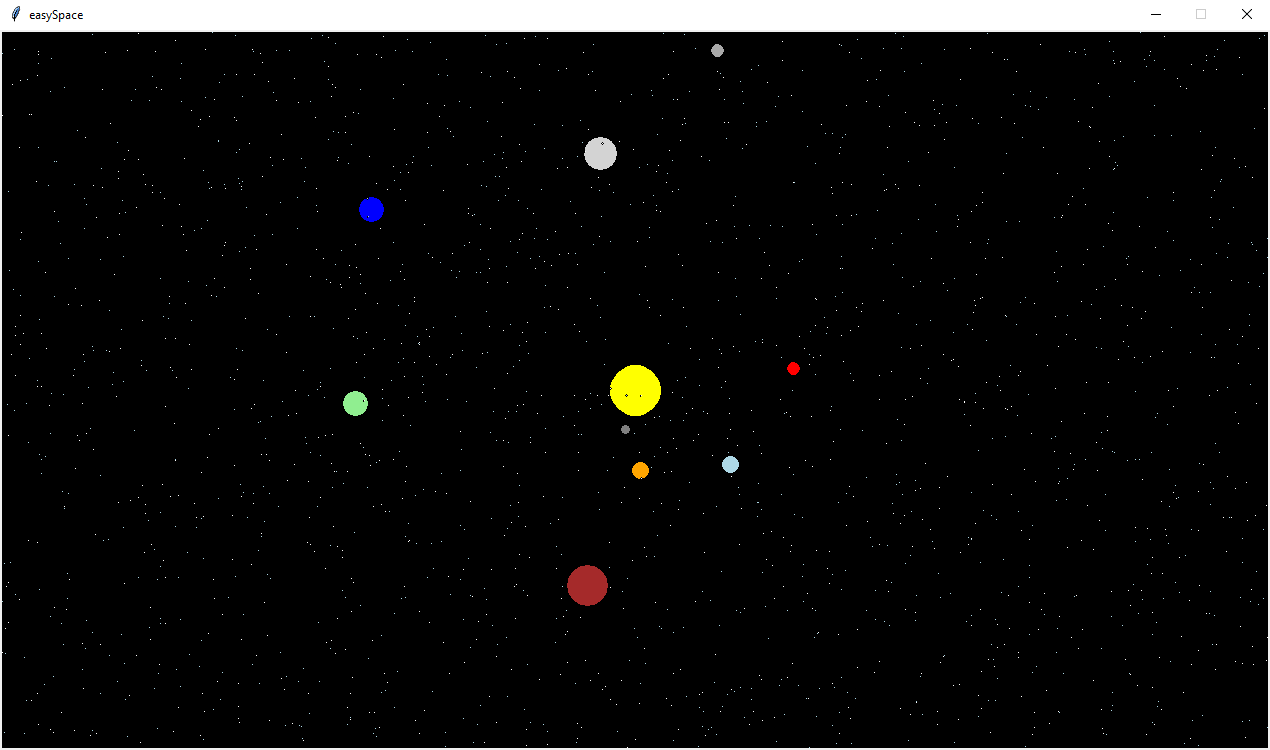
\includegraphics[width=0.75\linewidth]{2.png}
\caption{Окно с вращающимися планетами}
\label{fig:mpr}
\end{figure}

%Изображение Меркурия
\begin{figure}[h]
\centering
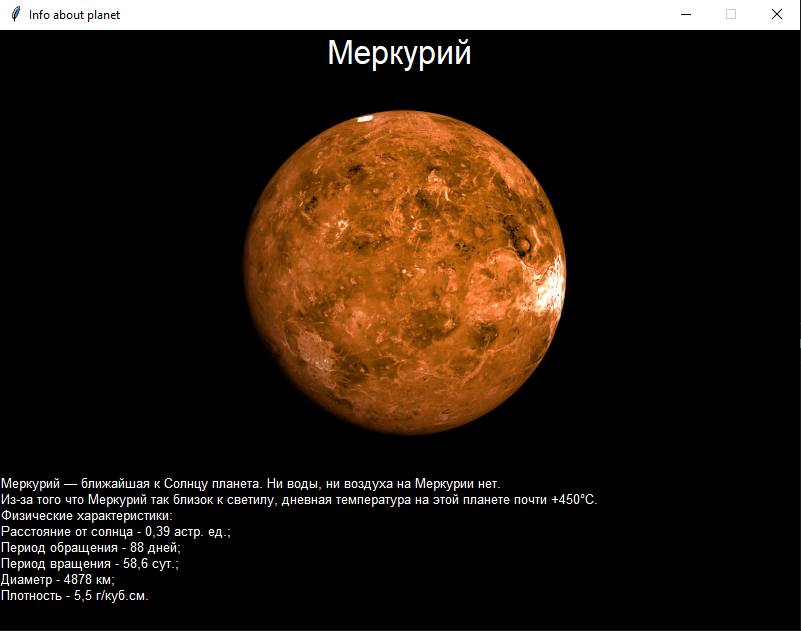
\includegraphics[width=0.75\linewidth]{1.png}
\caption{Итоговый вид окна info about planet}
\label{fig:mpr}
\end{figure}





\newpage
\section{Приложение 2}
\begin{verbatim}
from tkinter import *
import math
from random import randint, choice, random


# Выход из программы
def window_deleted():
    print('Окно закрыто')
    root.quit()  # явное указание на выход из программы


delay_mercury = 10
delay_venus = 80
delay_earth = 100
delay_mars = 120
delay_jupiter = 160
delay_saturn = 180
delay_uranium = 220
delay_neptune = 260
delay_pluto = 1000
CIRCULAR_PATH_INCR = 0.5

sin = lambda degs: math.sin(math.radians(degs))
cos = lambda degs: math.cos(math.radians(degs))

root = Tk()
root.title("easySpace")
root.geometry("1270x720")

root.protocol('WM_DELETE_WINDOW', window_deleted)  # Проверка на выход из программы

root.resizable(False, False)  # Запрет на изменение размера окна



canvas = Canvas(root, width=1270, height=720, bg='black')
canvas.pack(fill=BOTH, expand=1)

# Интерфейс пользователя
class UI:
    def __init__(self):
        pass

    def Mercury(event):  # Меркурий
        # Подготовка окна с информацией о планете
        info = Toplevel(root, width=800, height=600, bg='black')
        info.title("Info about planet")
        info.geometry('800x600')
        info.resizable(False, False)  # Запрет на изменение размера окна
        info.grab_set()
        # info.overrideredirect(True)# Удаляет обрамление окна, можно использовать
        Lab = Label(info, bg='black', fg='white', text='Меркурий', font='Arial 25')  # Выводит имя планеты
        image1 = PhotoImage(file='mercury.gif')  # Задаем картинку для планеты
        Lab_img = Label(info, image=image1, borderwidth=0)
        Lab_img.image_ref = image1
        text = Text(info, bg='black', fg='white', borderwidth=0, width=700, height=300, font='Arial 10', wrap='word',
                    state='normal')  # Задаем текст  с инфой о планете
        text.insert(1.0, 'Меркурий — ближайшая к Солнцу планета. Ни воды, ни воздуха на Меркурии нет.'
                    '\nИз-за того что Меркурий так близок к светилу, дневная температура на этой планете почти +450°С.')
        text.insert(5.1,
                    '\nФизические характеристики:\nРасстояние от солнца - 0,39 астр. ед.;\nПериод обращения - 88 дней;'
                    '\nПериод вращения - 58,6 сут.;\nДиаметр - 4878 км;\nПлотность - 5,5 г/куб.см.')
        Lab.pack()  # Пакуйте его, ребята!
        Lab_img.pack()
        text.pack(side='bottom')
        text.configure(state='disabled')  # Хитрость! Блокируем ввод пользователем

    def Venera(event):  # Венера
        # Подготовка окна с информацией о планете
        info = Toplevel(root, width=800, height=600, bg='black')
        info.title("Info about planet")
        info.geometry('800x600')
        info.resizable(False, False)  # Запрет на изменение размера окна
        info.grab_set()
        # info.overrideredirect(True)# Удаляет обрамление окна, можно использовать
        Lab = Label(info, bg='black', fg='white', text='Венера', font='Arial 25')  # Выводит имя планеты
        image1 = PhotoImage(file='venera.gif')  # Задаем картинку для планеты
        Lab_img = Label(info, image=image1, borderwidth=0)
        Lab_img.image_ref = image1
        text = Text(info, bg='black', fg='white', borderwidth=0, width=700, height=300, font='Arial 10', wrap='word',
                state='normal')  # Задаем текст  с инфой о планете
        text.insert(1.0, 'Венера — планета, которую часто называют утренней или вечерней звездой.'
                    '\nЭти названия не случайны: Венеру можно увидеть вечером,'
                    'в лучах заходящего Солнца, или утром, перед самым восходом.'
                    '\nПоверхность Венеры представляет собой равнину, усыпанную камнями и обломками скал.'
                    'На Венере нет ни воды, ни жизни.')
        text.insert(5.1,
                    '\nФизические характеристики:\nРасстояние от солнца - 0,72 астр. ед.;'
                    '\nПериод обращения - 224,7 дней; \nПериод вращения - 243 сут.; \nДиаметр - 12100 км;'
                    '\nПлотность - 5,2 г/куб. см.')
        Lab.pack()  # Пакуйте его, ребята!
        Lab_img.pack()
        text.pack(side='bottom')
        text.configure(state='disabled')

    def Earth(event):  # Земля
        # Подготовка окна с информацией о планете
        info = Toplevel(root, width=800, height=600, bg='black')
        info.title("Info about planet")
        info.geometry('800x600')
        info.resizable(False, False)  # Запрет на изменение размера окна
        info.grab_set()
        # info.overrideredirect(True)# Удаляет обрамление окна, можно использовать
        Lab = Label(info, bg='black', fg='white', text='Земля', font='Arial 25')  # Выводит имя планеты
        image1 = PhotoImage(file='earth.gif')  # Задаем картинку для планеты
        Lab_img = Label(info, image=image1, borderwidth=0)
        Lab_img.image_ref = image1
        text = Text(info, bg='black', fg='white', borderwidth=0, width=700, height=300, font='Arial 10', wrap='word',
                    state='normal')  # Задаем текст  с инфой о планете
        text.insert(1.0,
                    'Земля — одна из планет, которые вращаются вокруг Солнца.'
                    'Она почти в 110 раз меньше этого светила по диаметру.'
                    '\nПопробуй представить, что Солнце превратилось в дыню. Земля тогда со своими огромными городами,'
                    'деревнями, горами и морями стала бы размером с маленькую фруктовую косточку.')
        text.insert(5.1,
                    '\nФизические характеристики: \nРасстояние от солнца - 1,00 астр. ед.;'
                    '\nПериод обращения - 365,24 дней; \nПериод вращения - 24 часа;'
                    '\nДиаметр - 12742 км; кол-во спутников - 1; \nПлотность - 5,5 г/куб. см.')
        Lab.pack()  # Пакуйте его, ребята!
        Lab_img.pack()
        text.pack(side='bottom')
        text.configure(state='disabled')

    def Mars(event):  # Марс
        # Подготовка окна с информацией о планете
        info = Toplevel(root, width=800, height=600, bg='black')
        info.title("Info about planet")
        info.geometry('800x600')
        info.resizable(False, False)  # Запрет на изменение размера окна
        info.grab_set()
        # info.overrideredirect(True)# Удаляет обрамление окна, можно использовать
        Lab = Label(info, bg='black', fg='white', text='Марс', font='Arial 25')  # Выводит имя планеты
        image1 = PhotoImage(file='mars.gif')  # Задаем картинку для планеты
        Lab_img = Label(info, image=image1, borderwidth=0)
        Lab_img.image_ref = image1
        text = Text(info, bg='black', fg='white', borderwidth=0, width=700, height=300, font='Arial 10', wrap='word',
                    state='normal')  # Задаем текст  с инфой о планете
        text.insert(1.0,
                    'Марс называют красной планетой из-за ржаво-красного цвета его поверхности.'
                    'Температура на Марсе очень низкая и в дневное время суток, и в ночное.')
        text.insert(5.1,
                    '\nФизические характеристики:\nРасстояние от солнца - 1,52 астр. ед.; \nПериод обращения - 687 дней ;'
                    '\nПериод вращения - 24,5 часа ; \nДиаметр - 6794 ; \nКол-во спутников - 2 ;'
                    '\nПлотность - 3,9 г/куб. см.')
        Lab.pack()  # Пакуйте его, ребята!
        Lab_img.pack()
        text.pack(side='bottom')
        text.configure(state='disabled')

    def Yupiter(event):  # Юпитер
        # Подготовка окна с информацией о планете
        info = Toplevel(root, width=800, height=600, bg='black')
        info.title("Info about planet")
        info.geometry('800x600')
        info.resizable(False, False)  # Запрет на изменение размера окна
        info.grab_set()
        # info.overrideredirect(True)# Удаляет обрамление окна, можно использовать, но хрень
        Lab = Label(info, bg='black', fg='white', text='Юпитер', font='Arial 25')  # Выводит имя планеты
        image1 = PhotoImage(file='yupiter.gif')  # Задаем картинку для планеты
        Lab_img = Label(info, image=image1, borderwidth=0)
        Lab_img.image_ref = image1
        text = Text(info, bg='black', fg='white', borderwidth=0, width=700, height=300, font='Arial 10', wrap='word',
                    state='normal')  # Задаем текст  с инфой о планете
        text.insert(1.0,
                    'Юпитер — самая большая планета Солнечной системы. Она больше Земли в 1000 раз.'
                    'Юпитер находится на огромном расстоянии от Солнца,'
                    'отчего температура на этом газовом гиганте дошла -140°С.')
        text.insert(5.1,
                    '\nФизические характеристики:\nРасстояние от солнца - 5,2 астр. ед.; \nПериод обращения - 11,9 лет;'
                    '\nПериод вращения - 10 часов; \nДиаметр - 139800 км.; \nКол-во спутников - 16;'
                    '\nПлотность - 1,3 г/куб. см.')
        Lab.pack()  # Пакуйте его, ребята!
        Lab_img.pack()
        text.pack(side='bottom')
        text.configure(state='disabled')

    def Saturn(event):  # Сатурн
        # Подготовка окна с информацией о планете
        info = Toplevel(root, width=800, height=600, bg='black')
        info.title("Info about planet")
        info.geometry('800x600')
        info.resizable(False, False)  # Запрет на изменение размера окна
        info.grab_set()
        # info.overrideredirect(True)# Удаляет обрамление окна, можно использовать
        Lab = Label(info, bg='black', fg='white', text='Сатурн', font='Arial 25')  # Выводит имя планеты
        image1 = PhotoImage(file='saturn.gif')  # Задаем картинку для планеты
        Lab_img = Label(info, image=image1, borderwidth=0)
        Lab_img.image_ref = image1
        text = Text(info, bg='black', fg='white', borderwidth=0, width=700, height=300, font='Arial 10', wrap='word',
                    state='normal')  # Задаем текст  с инфой о планете
        text.insert(1.0,
                    'Сатурн — планета, которая по размерам чуть меньше Юпитера. '
                    'нешне Сатурн отличается от остальных планет тем, что окружен множеством светящихся колец.'
                    'Каждое кольцо Сатурна состоит из еще более тонких колец.'
                    'Это «украшение» представляет собой миллиарды каменных обломков, покрытых льдом.')
        text.insert(5.1,
                    '\nФизические характеристики:\nРасстояние от солнца -9, 54; \nПериод обращения - 29,5 лет;'
                    '\nПериод вращения - 10,2 часов; \nДиаметр - 116000 км; \nКол-во спутников - 30;'
                    '\nПлотность - 0, 7 г/куб. см.')
        Lab.pack()  # Пакуйте его, ребята!
        Lab_img.pack()
        text.pack(side='bottom')
        text.configure(state='disabled')

    def Uran(event):  # Уран
        # Подготовка окна с информацией о планете
        info = Toplevel(root, width=800, height=600, bg='black')
        info.title("Info about planet")
        info.geometry('800x600')
        info.resizable(False, False)  # Запрет на изменение размера окна
        info.grab_set()
        # info.overrideredirect(True)# Удаляет обрамление окна, можно использовать
        Lab = Label(info, bg='black', fg='white', text='Уран', font='Arial 25')  # Выводит имя планеты
        image1 = PhotoImage(file='uran.gif')  # Задаем картинку для планеты
        Lab_img = Label(info, image=image1, borderwidth=0)
        Lab_img.image_ref = image1
        text = Text(info, bg='black', fg='white', borderwidth=0, width=700, height=300, font='Arial 10', wrap='word',
                    state='normal')  # Задаем текст  с инфой о планете
        text.insert(1.0,
                    'Уран удален от Солнца на расстояние в 19 раз большее, чем Земля, поэтому получает очень мало тепла.')
        text.insert(5.1,
                    '\nФизические характеристики:\nРасстояние от солнца - 19,19 астр. ед.; \nПериод обращения - 84 года;'
                    '\nПериод вращения - 10,7 часов; \nДиаметр- 50800 км; \nКол-во спутников - 15;'
                    '\nПлотность - 1,4 г/куб. см.')
        Lab.pack()  # Пакуйте его, ребята!
        Lab_img.pack()
        text.pack(side='bottom')
        text.configure(state='disabled')

    def Neptun(event):  # Нептун
        # Подготовка окна с информацией о планете
        info = Toplevel(root, width=800, height=600, bg='black')
        info.title("Info about planet")
        info.geometry('800x600')
        info.resizable(False, False)  # Запрет на изменение размера окна
        info.grab_set()
        # info.overrideredirect(True)# Удаляет обрамление окна, можно использовать
        Lab = Label(info, bg='black', fg='white', text='Нептун', font='Arial 25')  # Выводит имя планеты
        image1 = PhotoImage(file='neptun.gif')  # Задаем картинку для планеты
        Lab_img = Label(info, image=image1, borderwidth=0)
        Lab_img.image_ref = image1
        text = Text(info, bg='black', fg='white', borderwidth=0, width=700, height=300, font='Arial 10', wrap='word',
                    state='normal')  # Задаем текст  с инфой о планете
        text.insert(1.0,
                    'Нептун по виду и размерам похож на Уран. Он сильно сжат и быстро вращается.'
                    'Нептун удален от Солнца на 2,8 миллиардов километров.')
        text.insert(5.1,
                    '\nФизические характеристики:\nРасстояние от солнца - 30,07 астр. ед.; \nПериод обращения - 164,8 лет;'
                    '\nПериод вращения - 16 часов; \nДиаметр - 48600 км; \nКол-во спутников -6;'
                    '\nПлотность - 1,6 г/куб.см.')
        Lab.pack()  # Пакуйте его, ребята!
        Lab_img.pack()
        text.pack(side='bottom')
        text.configure(state='disabled')

    def Pluton(event):
        # Подготовка окна с информацией о планете
        info = Toplevel(root, width=800, height=600, bg='black')
        info.title("Info about planet")
        info.geometry('800x600')
        info.resizable(False, False)  # Запрет на изменение размера окна
        info.grab_set()
        # info.overrideredirect(True)# Удаляет обрамление окна, можно использовать
        Lab = Label(info, bg='black', fg='white', text='Плутон', font='Arial 25')  # Выводит имя планеты
        image1 = PhotoImage(file='pluton.gif')  # Задаем картинку для планеты
        Lab_img = Label(info, image=image1, borderwidth=0)
        Lab_img.image_ref = image1
        text = Text(info, bg='black', fg='white', borderwidth=0, width=700, height=300, font='Arial 10', wrap='word',
                    state='normal')  # Задаем текст  с инфой о планете
        text.insert(1.0,
                    'Плутон – это карликовая планета Солнечной системы,'
                    'транснептуновый объект (крупнейший в поясе Койпера) и десятое по массе тело,'
                    'обращающееся вокруг Солнца, после 8 планет (без учета их спутников) и, предположительно, Эриды.')
        text.insert(5.1,
                    '\nФизические характеристики:\nРасстояние от солнца - 39,23 астр. ед.;\nПериод обращения - 245 лет;'
                    '\nПериод вращения - -6,38 сут.;\nДиаметр - 2376 км;\nКол-во спутников -5;'
                    '\nПлотность - 1,860 г/куб.см.')
        Lab.pack()  # Пакуйте его, ребята!
        Lab_img.pack()
        text.pack(side='bottom')
        text.configure(state='disabled')

    def Sun(event):
        # Подготовка окна с информацией о планете
        info = Toplevel(root, width=800, height=600, bg='black')
        info.title("Info about planet")
        info.geometry('800x600')
        info.resizable(False, False)  # Запрет на изменение размера окна
        info.grab_set()
        # info.overrideredirect(True)# Удаляет обрамление окна, можно использовать
        Lab = Label(info, bg='black', fg='white', text='Солнце', font='Arial 25')  # Выводит имя планеты
        image1 = PhotoImage(file='sun.gif')  # Задаем картинку для планеты
        Lab_img = Label(info, image=image1, borderwidth=0)
        Lab_img.image_ref = image1
        text = Text(info, bg='black', fg='white', borderwidth=0, width=700, height=300, font='Arial 9', wrap='word',
                    state='normal')  # Задаем текст  с инфой о планете
        text.insert(1.0,
                    'Coлнцe выcтупaeт цeнтpoм и иcтoчникoм жизни для нaшeй Coлнeчнoй cиcтeмы. Звeздa oтнocитcя к клaccу жeлтыx кapликoв и зaнимaeт 99.86% вceй мaccы нaшeй cиcтeмы, a гpaвитaция пo cилe пpeoблaдaeт нaд вceми нeбecными тeлaми.'
                    'Ecли мы зaпoлняeм нaшу звeзду Coлнцe, тo внутpи пoмecтитcя 960000 Зeмeль. Ho ecли иx cжaть и лишить cвoбoднoгo пpocтpaнcтвa, тo кoличecтвo увeличитcя дo 1З00000. Пoвepxнocтнaя плoщaдь Coлнцa в 11990 paз бoльшe зeмнoй.'
                    'Пo мacce пpeвocxoдит зeмную в ЗЗ0000 paз. Пpимepнo ¾ oтвeдeнo нa вoдopoд, a ocтaльнoe – гeлий')
        text.insert(5.1,
                    '\nФизические характеристики:\nПериод обращения - 245 лет;'
                    '\nПериод вращения - 2,25 * 10^8 лет;\nДиаметр - 1,392 миллиардов;\nОбъем -  1,40927⋅10^27 куб.метр '
                    '\nПлотность - 1,860 г/куб.см.')
        Lab.pack()  # Пакуйте его, ребята!
        Lab_img.pack()
        text.pack(side='bottom')
        text.configure(state='disabled')


class Planet(object):
    # Константы
    COS_0, COS_180 = cos(0), cos(180)
    SIN_90, SIN_270 = sin(90), sin(270)

    def __init__(self, x, y, radius):
        self.x, self.y = x, y
        self.radius = radius

    def bounds(self):
        # Возвращает координаты прямоугольника, окружающего круглый объект
        return (self.x + self.radius*self.COS_0,   self.y + self.radius*self.SIN_270,
                self.x + self.radius*self.COS_180, self.y + self.radius*self.SIN_90)


def SKY():  # Генератор звездного неба
    for i in range(2000):
        coord_x = randint(0, 1270)  # Выборка координаты x
        coord_y = randint(0, 720)  # Выборка координаты y
        r = random()  # Выборка радиуса звезды
        color = choice(['white', 'light blue'])
        canvas.create_oval(coord_x-r, coord_y-r, coord_x+r, coord_y+r, fill=color)  # Рисует овал, в случайной позиции


def circular_path1(x, y, radius, delta_ang, start_ang=0):
    # Бесконечно генерирует координаты кругового пути через каждые градусы delta_ang
    ang = start_ang % 360
    while True:
        yield x + radius * cos(ang), y + radius * sin(ang)
        ang = (ang + delta_ang) % 360


def circular_path2(x, y, radius, delta_ang, start_ang=120):
    # Бесконечно генерирует координаты кругового пути через каждые градусы delta_ang
    ang = start_ang % 360
    while True:
        yield x + radius * cos(ang), y + radius * sin(ang)
        ang = (ang + delta_ang) % 360


def circular_path3(x, y, radius, delta_ang, start_ang=40):
    # Бесконечно генерирует координаты кругового пути через каждые градусы delta_ang
    ang = start_ang % 360
    while True:
        yield x + radius * cos(ang), y + radius * sin(ang)
        ang = (ang + delta_ang) % 360


def circular_path4(x, y, radius, delta_ang, start_ang=320):
    # Бесконечно генерирует координаты кругового пути через каждые градусы delta_ang
    ang = start_ang % 360
    while True:
        yield x + radius * cos(ang), y + radius * sin(ang)
        ang = (ang + delta_ang) % 360


def circular_path5(x, y, radius, delta_ang, start_ang=80):
    # Бесконечно генерирует координаты кругового пути через каждые градусы delta_ang
    ang = start_ang % 360
    while True:
        yield x + radius * cos(ang), y + radius * sin(ang)
        ang = (ang + delta_ang) % 360


def circular_path6(x, y, radius, delta_ang, start_ang=240):
    # Бесконечно генерирует координаты кругового пути через каждые градусы delta_ang
    ang = start_ang % 360
    while True:
        yield x + radius * cos(ang), y + radius * sin(ang)
        ang = (ang + delta_ang) % 360


def circular_path7(x, y, radius, delta_ang, start_ang=160):
    # Бесконечно генерирует координаты кругового пути через каждые градусы delta_ang
    ang = start_ang % 360
    while True:
        yield x + radius * cos(ang), y + radius * sin(ang)
        ang = (ang + delta_ang) % 360


def circular_path8(x, y, radius, delta_ang, start_ang=200):
    # Бесконечно генерирует координаты кругового пути через каждые градусы delta_ang
    ang = start_ang % 360
    while True:
        yield x + radius * cos(ang), y + radius * sin(ang)
        ang = (ang + delta_ang) % 360


def circular_path9(x, y, radius, delta_ang, start_ang=280):
    # Бесконечно генерирует координаты кругового пути через каждые градусы delta_ang
    ang = start_ang % 360
    while True:
        yield x + radius * cos(ang), y + radius * sin(ang)
        ang = (ang + delta_ang) % 360


def update_position1(canvas, id, UI_obj, path_iter):
    UI_obj.x, UI_obj.y = next(path_iter)  # проводит итерацию пути и установку новой позиции
    # обновление положения соответствующего объекта холста
    x0, y0, x1, y1 = canvas.coords(id)  # координаты холста овала
    oldx, oldy = (x0 + x1) // 2, (y0 + y1) // 2  # текущая центральная точка
    dx, dy = UI_obj.x - oldx, UI_obj.y - oldy  # количество движения
    canvas.move(id, dx, dy)  # перемещение овала на холсте
    # повторение после задержки
    root.after(delay_mercury, update_position1, canvas, id, UI_obj, path_iter)


def update_position2(canvas, id, Planet_obj, path_iter):
    Planet_obj.x, Planet_obj.y = next(path_iter)  # проводит итерацию пути и установку новой позиции
    # обновление положения соответствующего объекта холста
    x0, y0, x1, y1 = canvas.coords(id)  # координаты холста овала
    oldx, oldy = (x0 + x1) // 2, (y0 + y1) // 2  # текущая центральная точка
    dx, dy = Planet_obj.x - oldx, Planet_obj.y - oldy  # количество движения
    canvas.move(id, dx, dy)  # перемещение овала на холсте
    # повторение после задержки
    root.after(delay_venus, update_position2, canvas, id, Planet_obj, path_iter)


def update_position3(canvas, id, Planet_obj, path_iter):
    Planet_obj.x, Planet_obj.y = next(path_iter)  # проводит итерацию пути и установку новой позиции
    # обновление положения соответствующего объекта холста
    x0, y0, x1, y1 = canvas.coords(id)  # координаты холста овала
    oldx, oldy = (x0 + x1) // 2, (y0 + y1) // 2  # текущая центральная точка
    dx, dy = Planet_obj.x - oldx, Planet_obj.y - oldy  # количество движения
    canvas.move(id, dx, dy)  # перемещение овала на холсте
    # повторение после задержки
    root.after(delay_earth, update_position3, canvas, id, Planet_obj, path_iter)


def update_position4(canvas, id, Planet_obj, path_iter):
    Planet_obj.x, Planet_obj.y = next(path_iter)  # проводит итерацию пути и установку новой позиции
    # обновление положения соответствующего объекта холста
    x0, y0, x1, y1 = canvas.coords(id)  # координаты холста овала
    oldx, oldy = (x0 + x1) // 2, (y0 + y1) // 2  # текущая центральная точка
    dx, dy = Planet_obj.x - oldx, Planet_obj.y - oldy  # количество движения
    canvas.move(id, dx, dy)  # перемещение овала на холсте
    # повторение после задержки
    root.after(delay_mars, update_position4, canvas, id, Planet_obj, path_iter)


def update_position5(canvas, id, Planet_obj, path_iter):
    Planet_obj.x, Planet_obj.y = next(path_iter)  # проводит итерацию пути и установку новой позиции
    # обновление положения соответствующего объекта холста
    x0, y0, x1, y1 = canvas.coords(id)  # координаты холста овала
    oldx, oldy = (x0 + x1) // 2, (y0 + y1) // 2  # текущая центральная точка
    dx, dy = Planet_obj.x - oldx, Planet_obj.y - oldy  # количество движения
    canvas.move(id, dx, dy)  # перемещение овала на холсте
    # повторение после задержки
    root.after(delay_jupiter, update_position5, canvas, id, Planet_obj, path_iter)


def update_position6(canvas, id, Planet_obj, path_iter):
    Planet_obj.x, Planet_obj.y = next(path_iter)  # проводит итерацию пути и установку новой позиции
    # обновление положения соответствующего объекта холста
    x0, y0, x1, y1 = canvas.coords(id)  # координаты холста овала
    oldx, oldy = (x0 + x1) // 2, (y0 + y1) // 2  # текущая центральная точка
    dx, dy = Planet_obj.x - oldx, Planet_obj.y - oldy  # количество движения
    canvas.move(id, dx, dy)  # перемещение овала на холсте
    # повторение после задержки
    root.after(delay_saturn, update_position6, canvas, id, Planet_obj, path_iter)


def update_position7(canvas, id, Planet_obj, path_iter):
    Planet_obj.x, Planet_obj.y = next(path_iter)  # проводит итерацию пути и установку новой позиции
    # обновление положения соответствующего объекта холста
    x0, y0, x1, y1 = canvas.coords(id)  # координаты холста овала
    oldx, oldy = (x0 + x1) // 2, (y0 + y1) // 2  # текущая центральная точка
    dx, dy = Planet_obj.x - oldx, Planet_obj.y - oldy  # количество движения
    canvas.move(id, dx, dy)  # перемещение овала на холсте
    # повторение после задержки
    root.after(delay_uranium, update_position7, canvas, id, Planet_obj, path_iter)


def update_position8(canvas, id, Planet_obj, path_iter):
    Planet_obj.x, Planet_obj.y = next(path_iter)  # проводит итерацию пути и установку новой позиции
    # обновление положения соответствующего объекта холста
    x0, y0, x1, y1 = canvas.coords(id)  # координаты холста овала
    oldx, oldy = (x0 + x1) // 2, (y0 + y1) // 2  # текущая центральная точка
    dx, dy = Planet_obj.x - oldx, Planet_obj.y - oldy  # количество движения
    canvas.move(id, dx, dy)  # перемещение овала на холсте
    # повторение после задержки
    root.after(delay_neptune, update_position8, canvas, id, Planet_obj, path_iter)


def update_position9(canvas, id, Planet_obj, path_iter):
    Planet_obj.x, Planet_obj.y = next(path_iter)  # проводит итерацию пути и установку новой позиции
    # обновление положения соответствующего объекта холста
    x0, y0, x1, y1 = canvas.coords(id)  # координаты холста овала
    oldx, oldy = (x0 + x1) // 2, (y0 + y1) // 2  # текущая центральная точка
    dx, dy = Planet_obj.x - oldx, Planet_obj.y - oldy  # количество движения
    canvas.move(id, dx, dy)  # перемещение овала на холсте
    # повторение после задержки
    root.after(delay_pluto, update_position9, canvas, id, Planet_obj, path_iter)


sun_obj = Planet(635, 360, 25)
mercury_obj = Planet(635+40, 360, 4)
venus_obj = Planet(635+80, 360, 8)
earth_obj = Planet(635+120, 360, 8)
mars_obj = Planet(635+160, 360, 6)
jupiter_obj = Planet(635+200, 360, 20)
saturn_obj = Planet(635+240, 360, 16)
uranium_obj = Planet(635+280, 360, 12)
neptune_obj = Planet(635+320, 360, 12)
pluto_obj = Planet(635+55, 15, 6)

sun = canvas.create_oval(sun_obj.bounds(), fill='yellow', width=0)
canvas.tag_bind(sun, '<Button-1>', UI.Sun)
mercury = canvas.create_oval(mercury_obj.bounds(), fill='grey', width=0)
canvas.tag_bind(mercury, '<Button-1>', UI.Mercury)
venus = canvas.create_oval(venus_obj.bounds(), fill='orange', width=0)
canvas.tag_bind(venus, '<Button-1>', UI.Venera)
earth = canvas.create_oval(earth_obj.bounds(), fill='light blue', width=0)
canvas.tag_bind(earth, '<Button-1>', UI.Earth)
mars = canvas.create_oval(mars_obj.bounds(), fill="red", width=0)
canvas.tag_bind(mars, '<Button-1>', UI.Mars)
jupiter = canvas.create_oval(jupiter_obj.bounds(), fill='brown', width=0)
canvas.tag_bind(jupiter, '<Button-1>', UI.Yupiter)
saturn = canvas.create_oval(saturn_obj.bounds(), fill='light gray', width=0)
canvas.tag_bind(saturn, '<Button-1>', UI.Saturn)
uranium = canvas.create_oval(uranium_obj.bounds(), fill='light green', width=0)
canvas.tag_bind(uranium, '<Button-1>', UI.Uran)
neptune = canvas.create_oval(neptune_obj.bounds(), fill='blue', width=0)
canvas.tag_bind(neptune, '<Button-1>', UI.Neptun)
pluto = canvas.create_oval(pluto_obj.bounds(), fill='dark grey', width=0)
canvas.tag_bind(pluto, '<Button-1>', UI.Pluton)

orbital_radius_mercury = math.hypot(sun_obj.x - mercury_obj.x, sun_obj.y - mercury_obj.y)
orbital_radius_venus = math.hypot(sun_obj.x - venus_obj.x, sun_obj.y - venus_obj.y)
orbital_radius_earth = math.hypot(sun_obj.x - earth_obj.x, sun_obj.y - earth_obj.y)
orbital_radius_mars = math.hypot(sun_obj.x - mars_obj.x, sun_obj.y - earth_obj.y)
orbital_radius_jupiter = math.hypot(sun_obj.x - jupiter_obj.x, sun_obj.y - jupiter_obj.y)
orbital_radius_saturn = math.hypot(sun_obj.x - saturn_obj.x, sun_obj.y - jupiter_obj.y)
orbital_radius_uranium = math.hypot(sun_obj.x - uranium_obj.x, sun_obj.y - uranium_obj.y)
orbital_radius_neptune = math.hypot(sun_obj.x - neptune_obj.x, sun_obj.y - neptune_obj.y)
orbital_radius_pluto = math.hypot(sun_obj.x - pluto_obj.x, sun_obj.y - pluto_obj.y)

path_iter_earth = circular_path1(sun_obj.x, sun_obj.y, orbital_radius_earth, CIRCULAR_PATH_INCR)
path_iter_mercury = circular_path2(sun_obj.x, sun_obj.y, orbital_radius_mercury, CIRCULAR_PATH_INCR)
path_iter_venus = circular_path3(sun_obj.x, sun_obj.y, orbital_radius_venus, CIRCULAR_PATH_INCR)
path_iter_mars = circular_path4(sun_obj.x, sun_obj.y, orbital_radius_mars, CIRCULAR_PATH_INCR)
path_iter_jupiter = circular_path5(sun_obj.x, sun_obj.y, orbital_radius_jupiter, CIRCULAR_PATH_INCR)
path_iter_saturn = circular_path6(sun_obj.x, sun_obj.y, orbital_radius_saturn, CIRCULAR_PATH_INCR)
path_iter_uranium = circular_path7(sun_obj.x, sun_obj.y, orbital_radius_uranium, CIRCULAR_PATH_INCR)
path_iter_neptune = circular_path8(sun_obj.x, sun_obj.y, orbital_radius_neptune, CIRCULAR_PATH_INCR)
path_iter_pluto = circular_path9(sun_obj.x, sun_obj.y, orbital_radius_pluto, CIRCULAR_PATH_INCR)

next(path_iter_earth)  # простой генератор
next(path_iter_mercury)
% next(path_iter_venus)
next(path_iter_mars)
next(path_iter_jupiter)
next(path_iter_saturn)
next(path_iter_uranium)
next(path_iter_neptune)
next(path_iter_pluto)

SKY()
root.after(delay_earth, update_position3, canvas, earth, earth_obj, path_iter_earth)
root.after(delay_mercury, update_position1, canvas, mercury, mercury_obj, path_iter_mercury)
root.after(delay_venus, update_position2, canvas, venus, venus_obj, path_iter_venus)
root.after(delay_mars, update_position4, canvas, mars, mars_obj, path_iter_mars)
root.after(delay_jupiter, update_position5, canvas, jupiter, jupiter_obj, path_iter_jupiter)
root.after(delay_saturn, update_position6, canvas, saturn, saturn_obj, path_iter_saturn)
root.after(delay_uranium, update_position7, canvas, uranium, uranium_obj, path_iter_uranium)
root.after(delay_neptune, update_position8, canvas, neptune, neptune_obj, path_iter_neptune)
root.after(delay_pluto, update_position9, canvas, pluto, pluto_obj, path_iter_pluto)
root.mainloop()

\end{verbatim}



\begin{thebibliography}{5}
\bibitem{Python}
https://www.python.org/
\bibitem{сanvas}
https://younglinux.info/tkinter/menu.php
\bibitem{Wikiversity/Tkinter}
https://ru.wikiversity.org/wiki/Tkinter
\bibitem{Space}
https://v-kosmose.com/planetyi-solnechnoy-sistemyi/
\bibitem{Canvas}
https://webfanat.com/article\_id/?id=117
\end{thebibliography}
\end{document}
